\documentclass[tikz,border=8pt]{standalone}
\usetikzlibrary{positioning,arrows.meta,shapes.geometric}
\begin{document}
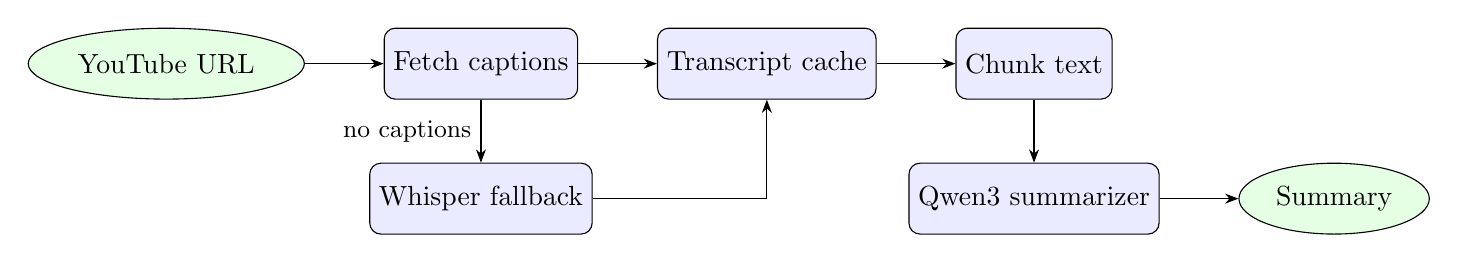
\begin{tikzpicture}[
  node distance=8mm and 10mm,
  proc/.style={rectangle, rounded corners, draw, fill=blue!8, minimum height=9mm, align=center},
  io/.style={ellipse, draw, fill=green!10, minimum height=9mm, align=center},
  >={Stealth}]
\node[io] (url) {YouTube URL};
\node[proc, right=of url] (cap) {Fetch captions};
\node[proc, below=of cap] (whisper) {Whisper fallback};
\node[proc, right=of cap] (cache) {Transcript cache};
\node[proc, right=of cache] (chunk) {Chunk text};
\node[proc, below=of chunk] (llm) {Qwen3 summarizer};
\node[io, right=of llm] (sum) {Summary};
\draw[->] (url) -- (cap);
\draw[->] (cap) -- (cache);
\draw[->] (cap) -- node[left, font=\small] {no captions} (whisper);
\draw[->] (whisper) -| (cache);
\draw[->] (cache) -- (chunk);
\draw[->] (chunk) -- (llm);
\draw[->] (llm) -- (sum);
\end{tikzpicture}
\end{document}
